% ExtremaFuse working manuscript. See README.md for the writing plan and evidence.
% FILL comments describe unfinished work. A dash in a table is an unreported value.
\documentclass[11pt]{article}
\usepackage[review]{acl}
\usepackage{times}
\usepackage{latexsym}
\usepackage[T1]{fontenc}
\usepackage[utf8]{inputenc}
\usepackage{microtype}
\usepackage{amsmath,amssymb,booktabs,graphicx}

\title{ExtremaFuse for Adaptive Compression of Frame-Level Speech Representations}
\author{Anonymous ACL submission}

\begin{document}
\maketitle

\begin{abstract}
How much can a recognizer shorten a speech sequence while retaining the distinctions needed to recognize phones? ExtremaFuse selects fusion centers at peaks and valleys of the cosine distance between adjacent frames and learns how to weight the five frames around each center. We apply it to Mel features and again inside an offline Conformer transducer trained on 460 hours of LibriSpeech. On test-clean, this system has a phone error rate of 5.69 percent, compared with 5.74 percent for a stride-four baseline with the same input projection width and a wider encoder. In one full CPU decoding pass it uses 38.3 percent less time. Relative to fusion at the Mel input alone, the second stage removes 59.8 percent of the remaining steps at a cost of 0.11 percentage points in phone error. Measured fusion weights show how neighboring frames still contribute to the shorter sequence.
% FILL after independent evaluation: update the quality and timing claims together. Add a pooling comparison only when the independently trained control is scored.
\end{abstract}

\section{Introduction}
\label{sec:intro}
A stride-four encoder represents every four input frames with one time step, whether those frames cover a steady vowel or straddle a transition. A phone recognizer offers a direct test of this choice. A system might emit a shorter sequence yet introduce deletions where a brief sound becomes hard to distinguish. Conversely, even a large reduction in frame count may buy little decoding time once the cost of selecting, fusing and searching is included.

We propose ExtremaFuse, a local operation on a sequence of frame vectors. Peaks and valleys in adjacent-frame distance determine where to emit a vector. The five frames around each selected position determine its value through learned weights. The operator can act on acoustic features or intermediate encoder states and takes no phone boundaries as input.

We ask two questions. First, within the decoding-time budget of a fixed-stride recognizer, what phone error rate can the adaptive system achieve? We compare systems that match the per-frame projection or the encoder width and measure time for the full decoding pass. Second, what does an additional round of compression cost after the Mel sequence has already been shortened? We count the steps and phone errors, inspect which input frames contribute to an output, and test a length-matched replacement in the same trained model. A breakdown by speaking rate reveals which edit types account for the difference in aggregate error.

\section{Related Work}
\label{sec:related}
\paragraph{Time reduction for speech models.}
Funnel pooling reduces the frame rate inside large speech encoders, and fixed-stride subsampling has been studied at both the input and the output of Whisper \citep{wang-etal-2024-massive,cho-etal-2026-stride}. Adaptive methods also exploit neighboring representations. A-ToMe merges adjacent transducer tokens based on the similarity of their attention keys \citep{li23i_interspeech}. In audio language models, \citet{bhati-etal-2025-compression} compare segmentation from adjacent-frame distances with uniform pooling, and \citet{xiang-etal-2026-need} study similarity-based merging at multiple depths. ExtremaFuse uses extrema in the distance curve as centers for overlapping, learned windows. This design lets us inspect which frames actually contribute to each output.

\paragraph{Local acoustic change and phone evaluation.}
Changes between neighboring features can provide cues for phonetic segmentation \citep{kreuk20_interspeech,yantosca-cheng-2025-phonotomizer}. Here the selected positions serve as fusion centers. Their value is assessed through recognition of the reference phone sequence. Work on phone realization illustrates the range of distinctions hidden by a single aggregate score \citep{bharadwaj-etal-2026-prism}. We therefore also examine substitutions, deletions and insertions.

\section{ExtremaFuse}
\label{sec:method}
\subsection{Sequence interface}
The input is an ordered sequence $H=(h_1,\ldots,h_T)$ of valid $D$-dimensional frames. The output has the same feature dimension and a content-dependent length $K\leq T$. Downstream layers consume the new length and mask.
Figure~\ref{fig:method} shows how the original frames enter both selection and fusion.

\begin{figure}[t]
\centering
\begin{tabular}{@{}l@{\quad}l@{}}
\toprule
Input & $H=(h_1,\ldots,h_T)$\\
Select & $H\longmapsto(d_1,\ldots,d_{T-1})\longmapsto C$\\
Fuse & $(H,C)\longmapsto(z_{c_1},\ldots,z_{c_K})$\\
\bottomrule
\end{tabular}
\caption{ExtremaFuse at one insertion site. Distances determine an ordered set $C$ of centers. Each $z_c$ pools the original features around that center with learned weights. The next stage receives $K$ frames of dimension $D$.}
\label{fig:method}
\end{figure}

\subsection{Selecting fusion centers}
For adjacent nonzero frames, define $d_t=1-\cos(h_t,h_{t+1})$. A peak at $p$ selects frame $p+1$, immediately after a locally large change in direction. A valley at $v$ selects frame $v$ at a locally small change. We merge duplicate positions and keep them in chronological order. If a nonempty sequence has no interior extremum, we use its first frame. The number of centers follows from the input, without a target retention rate.

\subsection{Learning local fusion weights}
For a center $c$, let $W_c$ contain its valid neighbors up to two positions away, including $c$. A two-layer network takes the five concatenated frame vectors, applies a 32-unit ReLU layer and predicts five logits. Inputs outside the sequence use the nearest endpoint for this prediction. The softmax weights are renormalized over valid positions for the output,
\begin{equation}
 z_c=\sum_{j\in W_c}\alpha_{cj}h_j,\quad
 \alpha_{cj}\geq 0,\quad \sum_{j\in W_c}\alpha_{cj}=1 .
 \label{eq:fusion}
\end{equation}
Overlapping windows allow one input to contribute to more than one output. The center-selection rule has no trainable parameters. Each insertion site learns its own fusion weights through the recognition objective.

\section{Experimental Setup}
\label{sec:setup}
\begin{table*}[t]
\centering
\small
\begin{tabular}{@{}lrrrrrrr@{}}
\toprule
& Input & Encoder & Params & \multicolumn{2}{c}{test-clean} & \multicolumn{2}{c}{test-other}\\
\cmidrule(lr){5-6}\cmidrule(l){7-8}
System & proj. & width & (M) & PER (\%) & RTF & PER (\%) & RTF\\
\midrule
Fixed stride 4 (E09) & 128 & 512 & 29.58 & 5.7427 & 0.03971 & -- & --\\
ExtremaFuse, Mel + layer 5 (E10) & 128 & 128 & 4.25 & 5.6882 & 0.02450 & -- & --\\
Fixed stride 4 (E01) & 32 & 128 & 4.21 & 6.1289 & 0.03116 & -- & --\\
Uniform pooling, Mel + layer 5 & 128 & 128 & -- & -- & -- & -- & --\\
\bottomrule
\end{tabular}
\caption{Phone recognition quality and CPU decoding cost. E09 defines the time budget and matches E10's input projection. E01 matches its encoder width. Both metrics are lower-is-better. Dashes mark pending measurements.}
\label{tab:systems}
\end{table*}

\begin{figure*}[t]
\centering
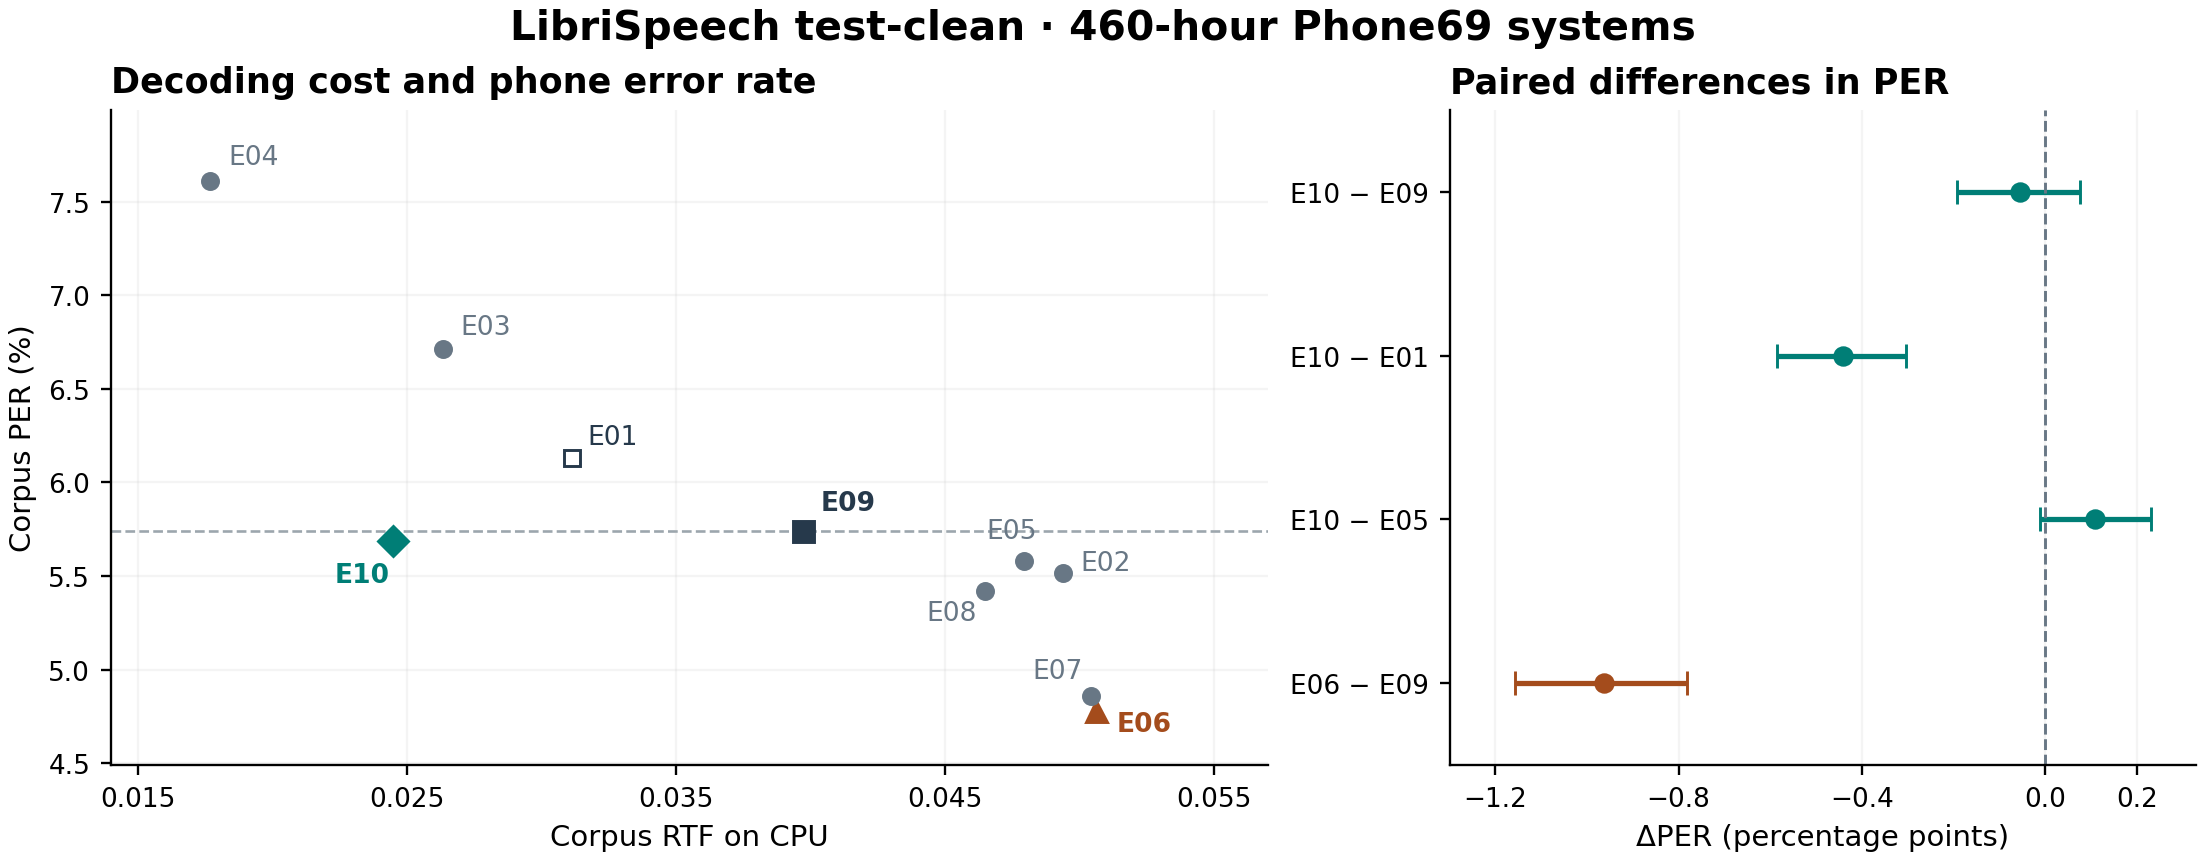
\includegraphics[width=\textwidth]{figures/quality_speed.png}
\caption{All ten observed test-clean configurations (left) and paired PER differences in percentage points (right). Points at or to the left of E09 meet its observed time budget. The horizontal line marks its PER. Intervals use 10,000 paired speaker resamples. Timing covers one complete decoding pass per system.}
\label{fig:operating}
\end{figure*}

\subsection{Task and systems}
We train on LibriSpeech train-clean-100 and train-clean-360 (460 hours) and recognize sequences from a 69-phone ARPABET inventory with vowel stress \citep{panayotov-etal-2015-librispeech}. We evaluate ExtremaFuse in a ten-layer offline Conformer with a transducer objective \citep{gulati20_interspeech,graves-2012-rnnt}. In the two-stage system (E10), fusion first shortens the 80-dimensional Mel sequence before its input projection. A second module acts after layer~5, so the final five encoder layers receive the twice-compressed sequence.

Four-frame stacking couples the input projection and encoder width in our baselines. E09 matches E10's 128-dimensional per-frame projection and stacks four projected vectors, giving it a 512-dimensional encoder. E01 uses a 32-dimensional projection to match E10's 128-dimensional encoder and approximate its parameter count (Table~\ref{tab:systems}). We train with seed 42 and select checkpoints by dev-clean validation loss. Batch budgets and update counts differ across runs. Appendix~\ref{app:configs} records the updates at selection and at the end of training.

\subsection{Uniform pooling control}
Uniform pooling tests whether comparable compression at the same sites suffices. The planned control uses E10's backbone and replaces both fusion modules with means over contiguous, disjoint segments of as nearly equal length as possible. At each site, its output length depends only on its input length and a retention ratio calibrated from E10 on dev-clean. The rest of the recognizer will be trained from scratch with these two ratios fixed.
% FILL after control training: record frozen ratios, realized per-stage frame totals, optimizer steps and any difference from E10's training schedule.

\subsection{Quality, cost, and uncertainty}
Corpus phone error rate (PER) divides total substitutions, deletions and insertions by the number of reference phones. We use the same 2,620 test-clean utterances for every system (189,023 phones, 40 speakers). Paired intervals resample speakers jointly across systems and recompute corpus PER on each of 10,000 draws. Test-clean informed the choice of configurations, so comparisons on this split are exploratory.

The real-time factor (RTF) divides total model decoding wall time by total audio duration. We evaluate the systems sequentially using four CPU compute threads, one inter-op thread, FP32, batch size one and beam width 20. Timing starts after feature preparation and covers the encoder, predictor, joiner and search. Ten warm-up utterances precede the timed pass. For the position study, a candidate meets the budget when its RTF divided by E09's RTF on the same split, device and decoding protocol is at most one.

We also plan to count major multiply--accumulate operations (MACs) per second of input audio. The counter uses each layer's actual sequence length and follows the hypotheses expanded by beam search. We will report encoder and compression MACs separately from predictor and joiner MACs, summing over utterances before dividing by total audio duration. Operations such as peak comparisons, sorting and memory access contribute to wall time outside this MAC count.

\begin{figure*}[t]
\centering
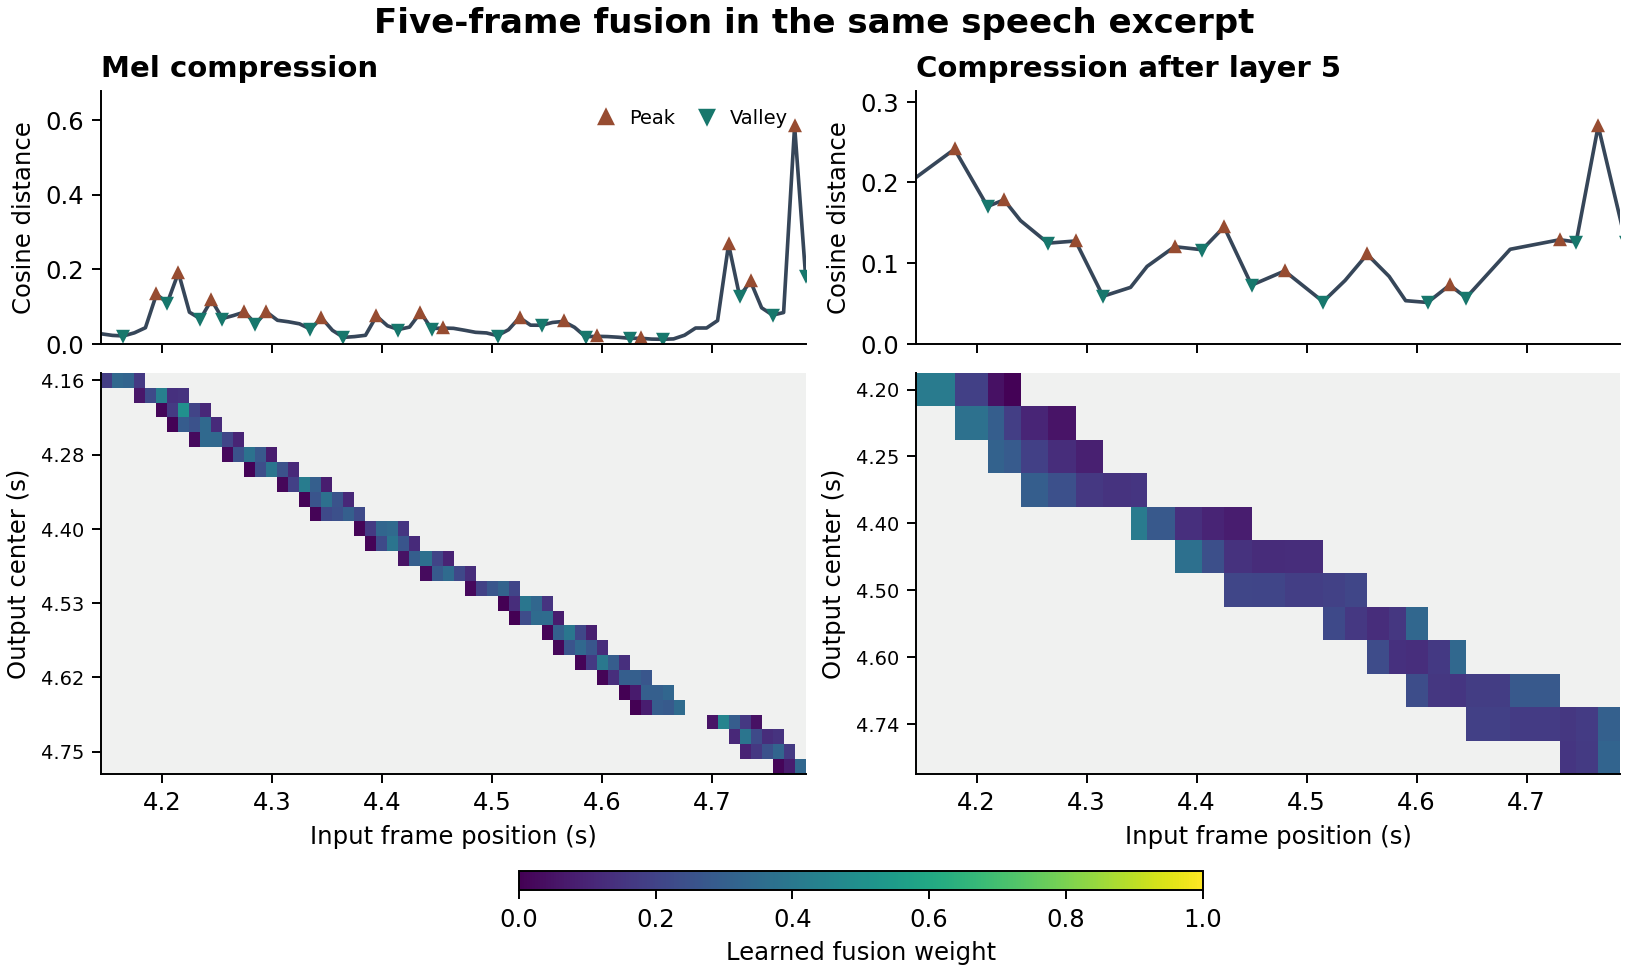
\includegraphics[width=0.90\textwidth]{figures/fusion_weights.png}
\caption{Measured distance curves and fusion weights for the same excerpt at the Mel input and after layer 5. Each row in the lower panels represents an output center. Layer-5 positions are expressed on the Mel time axis; their features already incorporate encoder context.}
\label{fig:weights}
\end{figure*}

\section{Results}
\label{sec:results}
\subsection{Recognition within the baseline time budget}
The two-stage system decoded test-clean at an RTF of 0.02450, against 0.03971 for E09, using 38.32\% less decoding time. The corresponding PERs were 5.6882\% and 5.7427\%. E10 made 103 fewer errors, a difference of $-0.054$ percentage points with a paired 95\% interval of $[-0.192,+0.076]$. The time saving is observed for these complete systems, which also differ in encoder width.

Matching the encoder width gives a second comparison. Relative to E01, E10 used 21.38\% less decoding time. Its PER difference was $-0.441$ percentage points, with a paired 95\% interval of $[-0.586,-0.303]$. The input projections and training budgets differ in this comparison. Of the ten measured systems, five met E09's observed time budget, including E09 itself. E10 had the lowest observed PER of those five. The fastest, E04, reached 0.01771 RTF at a PER of 7.6081\% (Figure~\ref{fig:operating}).

What do the one-stage systems achieve? Mel-only fusion (E05) gives a lower PER than E09 (5.5782\%) at a higher RTF (0.04795). Stride two with a single fusion after layer~2 (E03) reaches a lower RTF (0.02633) at a higher PER (6.7135\%). An alternative two-stage system (E08) also takes longer than E09. Among the measured alternatives, E10 alone improves both point estimates over E09. This observation leaves open whether a single fusion stage can also reach that operating point. We count adaptive fusion stages separately from fixed-stride stacking.

\subsection{Independent evaluation and pooling}
Two comparisons remain open. On test-other we will test whether E10 stays within a prespecified acceptable PER increase over E09. Repeated complete decoding passes, with system order balanced across rounds, will give the spread of their RTF ratio. We will also compare E10 with independently trained uniform pooling at the same two sites and report the realized frame counts, PER and RTF. The empty entries in Table~\ref{tab:systems} are reserved for these measurements.
% FILL independent quality: verify held-out use and phone-label coverage; fix the allowable loss in percentage points before scoring. Report E10-minus-E09 PER, its paired interval and whether its upper endpoint satisfies the margin.
% FILL repeated timing: alternate or counterbalance complete serial runs on the same CPU. Report paired E10/E09 RTF ratios across rounds, their spread and the number of rounds. Do not infer run-to-run variability from utterance resampling.
% FILL after full-corpus counting: give major MACs per audio second and their E09-relative ratios. Compare E02/E06 encoder work and search rows; use uninstrumented decoding for real-time claims.
% FILL trained pooling: compare both stages' retained fractions, paired PER and repeated RTF with E10. If pooling matches E10, say so when interpreting the contribution of adaptive fusion.

\section{Analysis}
\label{sec:analysis}
\subsection{The cost of the second fusion stage}
The fixed-stride baseline establishes the decoding budget. To examine the second compression itself, the relevant reference is the Mel-only system (E05). Across test-clean, both E05 and E10 produce 764,950 Mel-stage outputs. E10 reduces this to 307,404 steps after layer~5, removing a further 59.81\%. Its RTF falls from E05's 0.04795 to 0.02450, a 48.91\% reduction in decoding time.

E10 makes 208 more errors than E05. PER increases from 5.5782\% to 5.6882\%, a difference of $+0.110$ percentage points (paired 95\% interval $[-0.011,+0.232]$). These are separately trained systems. To test how much earlier the additional reduction can occur within the same time budget, Appendix~\ref{app:placement} reserves one paired comparison with the second stage after layer~2.

\subsection{Window coverage and a matched-length intervention}
\label{sec:weights}
Equation~\ref{eq:fusion} gives a bound on local distortion,
\begin{equation}
 \lVert z_c-h_c\rVert_2 \leq
 \sum_{j\in W_c}\alpha_{cj}\lVert h_j-h_c\rVert_2 .
 \label{eq:bound}
\end{equation}
When the neighbors receiving high weights resemble the center, the fused vector stays close to it. This gives a local explanation that can be checked against the actual inputs and weights. In 100 test-clean utterances (ten per speaking-rate decile, 37 speakers), adjacent vectors at layer~5 have a mean cosine similarity of 0.877. Pairs separated by half an utterance under a circular shift have a mean similarity of 0.143.

On this sample the second stage emits 40.19\% as many vectors as it receives. Its windows cover 98.24\% of the input positions, and 97.03\% receive a weight of at least 0.05 in at least one output. The effective number of inputs per output, $1/\sum_j\alpha_{cj}^2$, averages 3.89. Figure~\ref{fig:weights} shows how a frame between two centers can contribute to both. Coverage measures participation in fusion. Phone errors quantify which distinctions survive recognition.

Could an ordinary mean produce a similar result once the encoder has supplied context? We freeze E10, keep its Mel module, and replace only the layer-5 module with means over equally spaced segments. For every utterance we use exactly the number of outputs that E10 selected. Reference-transcript negative log-likelihood changes from 0.1423 to 0.1435 nats per phone (difference $+0.00117$, paired 95\% interval $[-0.00241,+0.00499]$). Thus the frozen model is also compatible with simple local averaging on this sample. The independently trained two-site control in Table~\ref{tab:systems} tests whether adaptive fusion improves recognition or decoding cost at a similar frame budget.

\subsection{Speaking rate and the error profile}
The small aggregate PER difference hides a change in error type. Across test-clean, E10 makes 832 fewer deletions than E09, alongside 235 more substitutions and 494 more insertions. To locate these changes, we group utterances by reference phones per minute of audio, including pauses. The slow and fast groups each contain three deciles and the middle group contains four.

\begin{table}[t]
\centering
\small
\begin{tabular}{@{}lrrrrr@{}}
\toprule
Group & Phones & $\Delta$S & $\Delta$D & $\Delta$I & $\Delta$PER\\
\midrule
Slow   & 36,624 & $+55$ & $-2$   & $-40$  & $+0.035$\\
Middle & 83,207 & $+95$ & $-326$ & $+279$ & $+0.058$\\
Fast   & 69,192 & $+85$ & $-504$ & $+255$ & $-0.237$\\
\bottomrule
\end{tabular}
\caption{E10 minus E09 on test-clean by speaking rate. S, D and I count substitutions, deletions and insertions. PER differences are in percentage points.}
\label{tab:rate}
\end{table}

The fast group accounts for 164 fewer errors, while the slow and middle groups contribute 13 and 48 additional errors (Table~\ref{tab:rate}). E10 retains similar proportions of the original Mel frames across the three groups (15.74\%, 15.77\% and 15.84\%). The fast-group PER difference is $-0.237$ percentage points (95\% interval $[-0.447,-0.010]$). Testing whether the benefit is larger in fast speech requires comparing groups directly. The fast-minus-slow difference is $-0.273$ percentage points with an interval of $[-0.697,+0.154]$, leaving the rate dependence uncertain.
% FILL held-out rate analysis: freeze thresholds on dev-clean, then report the same edit counts and fast-minus-slow interval on test-other.

\section{Conclusion}
\label{sec:conclusion}
On LibriSpeech test-clean, applying ExtremaFuse at the Mel input and inside the encoder gives a phone error rate close to the stride-four baseline while using 38.3\% less CPU decoding time in the measured pass. The second stage cuts the remaining sequence by more than half. Its overlapping windows still assign weight to most input positions, and the frozen model tolerates replacing them with length-matched averages on the diagnostic sample. Whether the learned rule adds value over trained uniform pooling is the open comparison most directly relevant to the method.
% FILL final conclusion: incorporate the held-out quality margin, repeated timing and trained pooling outcome, including a tie or a reversal.

\section*{Limitations}
Our evidence covers English read speech, phone recognition, one offline Conformer transducer and one training seed. The fixed-stride and adaptive systems differ in capacity or training exposure. The reported timing is specific to a batch-one CPU beam decoder and one full pass per system. The speaker intervals quantify test-sample uncertainty for these checkpoints. Test-clean was used to develop the comparisons, and the reference transcripts supply no aligned phone boundaries with which to score the selected centers.
% FILL: document the data used to estimate feature normalization when provenance is available.

\section*{Ethical Considerations}
% Optional ARR section. Fill verified corpus/label provenance, licensing and implications of stress or accent errors; remove this section if no additional discussion is included.
The evaluation uses English audiobook recordings and stressed phone labels. Application to other speaking styles or accents would require corresponding evaluation data.

% Omit acknowledgments in anonymous review. Use the separate ARR Responsible NLP Checklist for the applicable disclosures. Final acknowledgments belong before references.
\bibliography{references}

\appendix
\section{Configurations and Reproducibility}
\label{app:configs}
Table~\ref{tab:configs} gives the configurations behind Figure~\ref{fig:operating}. For E09 the validation loss selected an earlier checkpoint, at 23,150 of 117,500 updates. E10 was resumed with an increased phone-token batch budget and selected at 89,901 of 90,986 updates. Test scores throughout the paper correspond to the selected checkpoints.

\begin{table*}[t]
\centering
\small
\begin{tabular}{@{}llrrrrrr@{}}
\toprule
ID & Compression site(s) & Stride & Proj./width & Selected step & Final step & PER (\%) & RTF\\
\midrule
E01 & Fixed stride & 4 & 32/128 & 46,858 & 56,900 & 6.1289 & 0.03116\\
E02 & Layer 2 & 1 & 128/128 & 69,137 & 126,550 & 5.5141 & 0.04938\\
E03 & Layer 2 & 2 & 64/128 & 24,540 & 59,850 & 6.7135 & 0.02633\\
E04 & Layer 2 & 4 & 32/128 & 43,524 & 48,550 & 7.6081 & 0.01771\\
E05 & Mel & 1 & 128/128 & 121,688 & 126,550 & 5.5782 & 0.04795\\
E06 & Layer 5 & 1 & 128/128 & 151,700 & 165,000 & 4.7809 & 0.05062\\
E07 & Layer 7 & 1 & 128/128 & 118,826 & 126,550 & 4.8603 & 0.05042\\
E08 & Keep at 2, fuse at 5 & 1 & 128/128 & 73,182 & 141,382 & 5.4210 & 0.04649\\
E09 & Fixed stride & 4 & 128/512 & 23,150 & 117,500 & 5.7427 & 0.03971\\
E10 & Mel + layer 5 & 1 & 128/128 & 89,901 & 90,986 & 5.6882 & 0.02450\\
\bottomrule
\end{tabular}
\caption{Full test-clean comparison. For E08 the first stage keeps the union of each selected center and its immediate neighbors. The second applies learned five-frame fusion. Stride is the fixed stacking factor.}
\label{tab:configs}
\end{table*}

All systems use 16 kHz audio, 80 Mel bins and a 10 ms frame hop. Training uses Adam with a peak learning rate of 0.0005, 10,000 warm-up updates and gradient clipping at 10. The corpus bootstrap resamples 40 speakers with replacement using seed 42 and reports percentile intervals. All utterances from a sampled speaker enter each system's numerator and denominator together.
% FILL reproduction: provide anonymized recipes and checkpoint identifiers, feature-statistics provenance, CPU model, library versions and the repeated-round ordering.

\section{Additional Diagnostics}
\label{app:diagnostics}
\subsection{Testing early placements under the time budget}
\label{app:placement}
The stride-one, layer-2-only system (E02) already exceeds E09's test-clean RTF, despite placing compression early. Table~\ref{tab:early} reserves two early placements for distinct questions. A layer-1-only run would test a new one-stage candidate against both E02 and E09. A Mel-plus-layer-2 run could be compared with E02 to examine the addition of Mel fusion, and with E10 to examine moving the second module forward. In the latter comparison, layers~3 through~5 would also process the shortened sequence.

\begin{table}[t]
\centering
\small
\begin{tabular}{@{}lrrr@{}}
\toprule
Fusion site(s) & PER (\%) & RTF & RTF/E09\\
\midrule
Layer 2 (E02) & 5.5141 & 0.04938 & 1.243\\
Mel + layer 5 & 5.6882 & 0.02450 & 0.617\\
\midrule
Layer 1 only & -- & -- & --\\
Mel + layer 2 & -- & -- & --\\
\bottomrule
\end{tabular}
\caption{Early-placement comparisons on test-clean. Measured rows are E02 and E10. Dashes reserve optional experiments. An RTF ratio of 1 is the baseline time budget.}
\label{tab:early}
\end{table}

Both proposed runs use stride one and a 128-dimensional projection and encoder. Each would follow the corresponding reference training recipe, with the actual updates recorded. We would report stage input and output counts, paired PER and full-pass CPU RTF, including any over-budget result. Candidate selection would use the E09-relative budget on dev-clean before confirmation on test-other.
% FILL optional early placement only: for the single-stage question compare layer 1 with E02 and E09. For the two-stage question compare Mel + layer 2 with E02 and E10. Record held-out results only for frozen comparisons.

\subsection{Selection of the illustrated excerpt}
For the weight diagnostic we select ten utterances per test-clean speaking-rate decile using a deterministic hash of the utterance identifier. Figure~\ref{fig:weights} shows a 0.64-second window centered at the midpoint of the lowest-hash eligible utterance in decile five (at least 200 raw frames). The choice therefore does not use recognition errors or the appearance of the weights.
% FILL: ten-bin results, phone-level error breakdowns, and paired examples of an improvement and a regression using a stated selection rule.

\end{document}
